\chapter{Marco Teórico}
\label{chap:marcoteorico}

\section{Introducci\'on}

Para el an\'alisis de posibles colisiones es necesario evaluar de forma anticipada las trayectorias de todos los objetos que orbitan la Tierra y detectar los acercamientos de riesgo. Si la predicci\'on de las posiciones fuera exacta, este estudio s\'olo implicar\'ia un esfuerzo computacional a resolver. No obstante, el movimiento orbital de los objetos no es ideal y las posiciones medidas o estimadas siempre acarrean una indeterminaci\'on; ya sea por: errores en la medici\'on, errores en el modelo de determinaci\'on orbital o errores en los modelos de predicci\'on orbital. A su vez, las indeterminaciones son mayores cuando se trata de desechos espaciales.\\

La t\'ecnica de detecci\'on de encuentros, consiste en realizar propagaciones de las posiciones de todo el cat\'alogo a partir de un instante inicial, en intervalos que por lo general, abarcan una semana hacia el futuro y medir las distancias entre los objetos. Se define un volumen seguro rodeando al sat\'elite de inter\'es, y si alg\'un objeto externo se introduce dentro del volumen de riesgo, es decir, se acerca a una distancia m\'inima por debajo del umbral determinado, se considera una situaci\'on de riesgo. 
Esta metodolog\'ia no tiene en cuenta los errores en la determinaci\'on de la posici\'on de los objetos, y por lo general deriva en falsas alarmas, con las que se corre el riesgo de realizar maniobras innecesarias o que pueden poner en mayor peligro a la misi\'on.\\

Una vez identificado un encuentro, para un estudio m\'as exhaustivo de la situaci\'on, adem\'as de la m\'inima distancia de acercamiento o {\it{miss distance}}, se calcula la PoC.  Esta \'ultima ofrece un panorama m\'as completo ya que incorpora los errores en las posiciones a trav\'es de las matrices de covarianza.\\

Como ya mencionamos (Sec. \ref{subsec:estudiocolision}), en este trabajo nos enfocamos en analizar las situaciones de encuentro ya identificadas y en particular, aquellas que involucran a misiones operativas y desechos espaciales.\\

En este cap\'itulo, en primer lugar, se presentan las distintas maneras en que se determinan las posiciones de los objetos, dependiendo de si son misiones operativas o desechos.\\
La posici\'on de la misi\'on operativa y los errores asociados a la misma, la provee el departamento de din\'amica orbital (Sec. \ref{sec:posMision}).
La posici\'on de los desechos, s\'olo es posible conocerla, utilizamos los datos p\'ublicos que ofrece el comando de defensa norteamericano, \ac{NORAD} a trav\'es de su p\'agina Space-Track {\footnote{http://www.space-track.org}}. Las posiciones son publicadas en formato \ac{TLE} (Sec. \ref{subsec:tleformat}), sin errores asociados, y son propagadas hasta el momento del encuentro con el modelo SGP4  \citep{hoots1980models}, que tampoco ofrece informaci\'on sobre los errores de propagaci\'on. Se dedica un \'item para presentar el modelo de propagaci\'on SGP4 (Sec. \ref{subsec:sgp4model}) y se agrega en este espacio una breve descripci\'on de los sistemas de referencia con los que se trabaj\'o.\\

La siguiente secci\'on describe el tratamiento de errores. Para el estudio de la estimaci\'on de los errores en la posici\'on inicial, se detalla el m\'etodo de Osweiler \citep{osweiler} que permite la construcci\'on de las matrices de covarianza a partir de un conjunto de TLEs, cuando no se cuenta con datos m\'as precisos.\\

Una vez calculada la matriz de covarianza de errores, asociada a la posici\'on inicial, ser\'a necesario propagarla al instante predicho para el encuentro. Para ello se propone la implementaci\'on de una tabla con valores estad\'isticos inferidos del an\'alisis comparativo de efem\'erides precisas de la misi\'on operativa y las propagaciones de los TLE.\\

Contin\'ua la secci\'on que explica el algoritmo para el c\'alculo de la PoC y finalmente se describe en detalle, la forma en que se comunican los acercamientos de riesgo (Sec. \ref{sec:anuncio}), por ejemplo mediante \ac{CDM}.
% Incorporar los estados de alerta de Nasa. (texto de la aseguradora Britanica que me paso Juan ... bla de UNLAM.)


\section{La posici\'on de los objetos involucrados}{\label{sec:posMision}}
Al estudio de posiciones orbitales se lo puede dividir en tres etapas: medici\'on y/o rastreo, determinaci\'on orbital y propagaci\'on orbital.

\begin{itemize}
\itemsep0em
 \item {\bf{Medici\'on y/o rastreo:}} Abarca las mediciones desde Tierra, con radares, instrumentos \'opticos, l\'aser o doppler; y en el caso de las misiones operativas, sistemas de navegaci\'on abordo, como por ejemplo GPS (Global Positioning System).\\
 \item {\bf{Determinaci\'on Orbital:}} Consiste en la utilizaci\'on de modelos de la \'orbita, que incorporan las mediciones y datos del entorno espacial (atm\'osfera, radiaci\'on solar, etc ) para ajustar los par\'ametros del modelo. Son procesamientos que se realizan a posteriori y que ofrecen distintos grados de precisión seg\'un las consideraciones que se tengan en cuenta.\\
 \item {\bf{Propagaci\'on Orbital:}} Es el proceso mediante el cual, se extrapolan hacia el futuro las \'orbitas calculadas mediante determinaci\'on orbital.\\
\end{itemize}


En nuestro planteo de riesgos de colisi\'on entre misiones operativas y desechos espaciales, existen dos abordajes distintos respecto de las posiciones, ya que cada uno de los objetos involucrados utiliza metodolog\'ias y modelos diferentes.

\subsection{La posici\'on de la misi\'on operativa}

Con una misi\'on operativa se mantiene el contacto y se la puede comandar. Los sistemas de navegaci\'on abordo permiten un registro permanente de las posiciones y velocidades del sat\'elite. Esos registros se utilizan en los ajustes de los modelos de determinaci\'on orbital, que se realizan en procesamientos posteriores y se generan efem\'erides orbitales de mucha precisi\'on, cuyos errores resultan del propio procesamiento.\\

Para este trabajo se tuvo acceso a los productos orbitales de una misi\'on operativa, cuyas efem\'erides se plasman en archivos de texto plano, tabuladas cada un segundo, en el sistema de referencia verdadero de la fecha \ac{TOD}. Seg\'un se nos inform\'o, los mismos presentan errores del orden de  20 metros, (comunicaci\'on por mail).\\

Estas {efem\'erides precisas y sus errores asociados son las que deben utilizarse en los estudios de riesgo, no obstante, para los procesamientos de este trabajo, si bien fue posible contar con las efem\'erides precisas, no se tuvo acceso a datos de acercamientos de riesgos por motivos de confidencialidad. Raz\'on por la cual, las posiciones de todos los objetos se calcularon a partir de los TLE p\'ublicos y las efem\'erides precisas fueron utilizadas para el estudio de los errores de los TLE, en particular para la generaci\'on de la tabla con los valores estad\'isticos de las varianzas, que se utilizan para la propagaci\'on de errores al instante TCA, (Sec. \ref{subsec:tablaprop}). \\

\subsection{La posici\'on del desecho espacial}
El desecho espacial no tiene capacidades operativas, de manera que la \'unica forma de determinar su posici\'on es mediante las redes de rastreo descritas en la introducci\'on.\\

Como en Argentina no contamos con capacidad de rastreo, ARxCODE fue dise\~nado para obtener los datos de los desechos en el formato TLE, que publica NORAD, mediante el sitio web Space-Track.
Si bien son los datos m\'as completos y difundidos, utilizar estos datos acarrea errores muy importantes, y sobre todo desconocidos. Es por eso que debe implementarse alg\'un m\'etodo que permita estimarlos.\\

En las secciones siguientes se explicita el formato de los TLE y se describe el modelo SGP4 que permite la propagaci\'on de los mismos.\\

\subsection{Los archivos TLE}\label{subsec:tleformat}

El formato TLE es un modo hist\'orico de registro de datos orbitales de los objetos rastreados que orbitan la Tierra. Sus siglas  hacen referencia a las Dos L\'ineas (Two-Line) en las que se plasman los elementos orbitales medios, junto con datos adicionales, de un dado objeto, para un instante particular.

Como se detalla a continuación, en la primera l\'inea se encuentran los identificadores del objeto y el n\'umero de lanzamiento del año, el instante en el que fueron calculados los elementos, y parámetros de ajuste, como las derivadas de movimiento medio y el t\'ermino de frenado atmosf\'erico, BSTAR, que resultan necesarios para la propagación de los TLE con el modelo dinámico SGP4, (Sec. \ref{subsec:sgp4model}).

\begin{center}
\fbox{\parbox[b]{0.8\linewidth}{
Ejemplo de un TLE de la Estaci\'on Espacial Internacional (ISS) \\

\noindent
{\bf{1 25544U 98067A   08264.51782528 -.00002182  00000-0 -11606-4 0  2927\\
2 25544  51.6416 247.4627 0006703 130.5360 325.0288 15.72125391563537}}\\

{\bf{LINE 1 Primera línea del TLE}}\\
1   01–01   Número de línea    1\\
2   03–07   Número de satélite 25544\\
3   08–08   Clasificación      U\\
4   10–11   Identificador internacional (últimos dígitos del año de lanz.) 98\\
5   12–14   Identificador internacionl (número de lanzamiento del año)     067\\
6   15–17   Identificador internacional (piece of the launch)     A\\
7   19–20   Época del año (últimos dígitos del año)     08\\
8   21–32   Época (día del año y fracción de la porción de día)     264.51782528\\
9   34–43   Derivada primera del movimiento medio dividida por dos.   −.00002182\\
10  45–52   Derivada segunda del movimiento medio. 00000-0\\
11  54–61   BSTAR término de frenado atmosférico. -11606-4\\
12  63–63   El número 0. (originalmente traía el tipo de efemérides) 0\\
13  65–68   Número de set. I\\
14  69–69   Checksum (modulo 10)  7\\

{\bf{LINE 2 Segunda l\'inea del TLE}}\\
1   01–01   Número de línea    2\\
2   03–07   Númera de satélite 25544\\
3   09–16   Inclinación (grados)     51.6416\\
4   18–25   Ascención Recta del nodo ascendente. (grados)   247.4627\\
5   27–33   Excentricidad (parte decimal)  0006703\\
6   35–42   Argumento del Perigeo (grados) 130.5360\\
7   44–51   Anomalía Media (grados) 325.0288\\
8   53–63   Movimiento Medio (revoluciones por día) 15.72125391\\
9   64–68   Número de órbita (revoluciones)  56353\\
10  69–69   Checksum (modulo 10)  7\\
}}
\end{center}

En la segunda l\'inea se ubican los elementos orbitales cl\'asicos medios: inclinaci\'on, longitud del nodo, excentricidad, argumento del perigeo, anomal\'ia media y el movimiento medio, de donde se extrae el valor del semieje. En este punto es importante resaltar el hecho de que se trata de elementos medios, promediados bajo ciertos criterios y metodologías no siempre especificadas, de manera que no son una exacta analog\'ia con los elementos orbitales de la posici\'on real para el instante indicado.

\subsection{El propagador SGP4}\label{subsec:sgp4model}
De acuerdo a una rese\~na hist\'orica presentada por Hoots \citep{hootshistoria}, los or\'igenes del propagador SGP4 se remontan al a\~no 1960 en EE.UU, cuando se desarroll\'o el modelo General Simplificado de Perturbaciones SGP  ({\it{Simplified General Pertubations}}). Basado en los modelos anal\'iticos de predicci\'on orbital de Brouwer \citep{brouwer1959solution} y Kozai \citep{kozai1962second}, para su implementaci\'on, fue adaptado y modificado para evitar singularidades en \'orbitas particulares y para reducir el tiempo de c\'omputo. As\'i mismo se incluy\'o el efecto del frenado atmosf\'erico.\\

En 1964 se convirti\'o en el modelo de predicci\'on orbital principal del sistema de detecci\'on y rastreo de los Estados Unidos de Am\'erica.
Sin embargo, en 1969 la cantidad de objetos catalogados imped\'ian a las computadoras de la \'epoca procesar todos los t\'erminos del modelo, por lo que fue necesario desarrollar una nueva versi\'on m\'as simplificada, que result\'o en el propagador SGP4 que se puso en operatividad en el a\~no 1970.\\

Esta \'ultima simplificaci\'on (Lane and Hoots, 1979) consisti\'o en :\\
\begin{itemize}
 \item Retener s\'olo los principales t\'erminos que modelan el efecto secular que produce el frenado atmosf\'erico.
 \item Restringir el modelo gravitacional de Brower s\'olo a los t\'erminos de per\'iodo largo o corto, que no contengan a la excentricidad como factor.
\end{itemize}

La primera versi\'on liberada del c\'odigo fuente del propagador SGP4 se public\'o en el Spacetrack Report Number 3 \citep{spacetrackreport3}.\\

En 2004 Hoots et al. public\'o un documento completo con todas las ecuaciones (incluidas las correspondientes al modelo para espacio profundo); incorporando resonancias, las fuerzas que ejercen otros cuerpos, el frenado atmosf\'erico y otras perturbaciones en las t\'ecnicas matem\'aticas.\\

El propagador SGP4 es actualmente, el \'unico modelo para el mantenimiento del cat\'alogo de objetos a bajas alturas que orbitan la Tierra. 

\subsection{Sistemas de Referencia}\label{subsec:sistRef}

\subsubsection*{\ac{TEME}}
 Es un sistema inercial con origen en el centro de la Tierra, que utiliza como plano fundamental el Ecuador Verdadero. El eje {\it{x}} se ubica en el plano del Ecuador Verdadero y apunta en la direcci\'on del Equinoccio Medio, el eje {\it{y}} tambi\'en se ubica sobre el plano ecuatorial a $90^{\circ}$ del eje {\it{x}}, y el eje {\it{z}} apunta en la direcci\'on del eje de rotaci\'on de la Tierra, perpendicular al plano ecuatorial. Sus siglas hacen referencia a un Ecuador Verdadero y un Equinoccio Medio o \ac{TEME}. Si bien no es un sistema convencional estandarizado, es el sistema que utiliza NORAD para la generaci\'on y propagaci\'on de los TLE, por lo que se encuentra ampliamente difundido.
 
\subsubsection*{True of Date (TOD)}}
 Al igual que el TEME, es un sistema inercial definido con origen en el centro de la Tierra, con plano fundamental el Ecuador Verdadero. Su eje {\it{x}} tambi\'en yace sobre el plano ecuatorial pero se orienta en la direcci\'on del Equinoccio Verdadero (de la fecha).\\
 En el Ap\'endice \ref{App1} se describe en forma detallada la transformaci\'on de coordenadas del sistema TEME al sistema TOD.
 
\subsubsection*{Sistemas centrados en el objeto}
Los sistemas \ac{RSW} y \ac{NTW} son dos sistemas con origen centrado en el objeto (Figura \ref{fig:sistref}). Esta caracter\'istica ofrece ventajas cuando se hacen estudios de movimientos relativos, como en las misiones de sistemas distribuidos, o en los acoplamientos entre naves y tambi\'en aclaran la influencia de ciertos efectos perturbadores, como por ejemplo el del frenado atmosf\'erico, muy notorio en la componente a lo largo de la velocidad.\\

\begin{figure}[!h]
\centering
\fbox{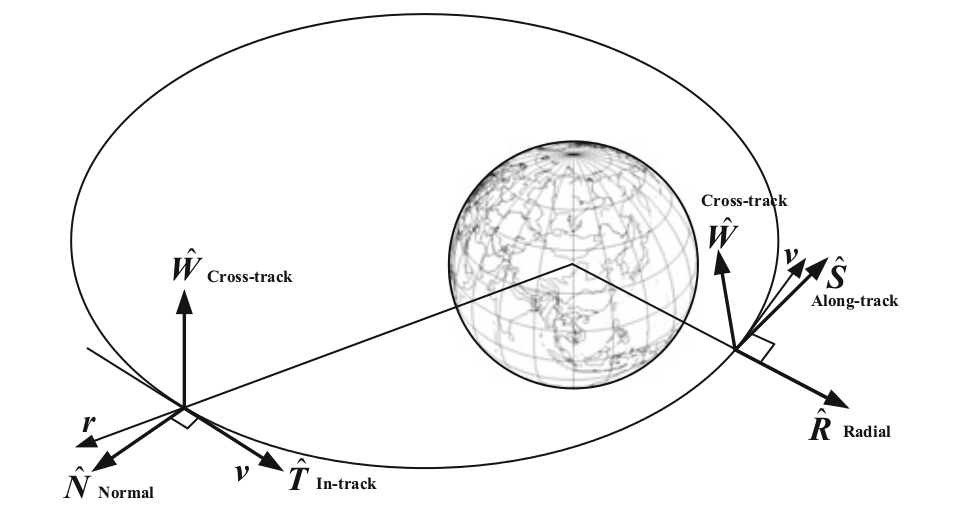
\includegraphics[width=0.8\textwidth]{imagenes/sistref}}
\caption[Sistemas de Referencia centrados en el Sat\'elite]{Sistemas de Referencia centrados en el Sat\'elite - extra\'ido de \cite{leichen}}
\label{fig:sistref}
\end{figure}


En el sistema {\bf{RSW}} la coordenada R (radial), tiene la direcci\'on del vector que une el centro de la Tierra con el objeto; la coordenada S ({\it{along-track or transverse}}), apunta en la direcci\'on perpendicular al vector R, a lo largo del movimiento pero no exactamente paralela a la direcci\'on de la velocidad (salvo en \'orbitas circulares o en \'orbitas el\'ipticas durante el apogeo y el perigeo); la coordenada W ({\it{cross-track}}), es perpendicular tanto a R como a S, es decir, normal al plano del movimiento. Este sistema tambi\'en se encuentra en la bibliograf\'ia como UVW, o \ac{RTN}.\\

Dado el vector posici\'on $\bar{r}$ y velocidad $\bar{v}$ del objeto de referencia, en un sistema inercial, en un momento dado; el sistema {\bf{RSW}} queda definido a partir de:\\


\begin{equation}
 \bar{R}=\frac{\bar{r}}{|\bar{r}|}, \quad \bar{W}=\frac{\bar{r}\times\bar{v}}{|\bar{r}\times\bar{v}|}, \quad \bar{S}=\bar{W}\times\bar{R}
\end{equation}

El sistema {\bf{NTW}} define el eje T (tangencial a la \'orbita) en la direcci\'on de la velocidad ({\it{in-track}}); el eje N (normal), en el plano orbital y perpendicular a la velocidad; y la componente W apunta en la direcci\'on perpendicular al plano orbital.\\

Dado el vector posici\'on $\bar{r}$ y velocidad $\bar{v}$ del objeto de referencia, en un sistema inercial, en un momento dado; el sistema {\bf{NTW}} queda definido a partir de:\\

\begin{equation}
 \bar{T}=\frac{\bar{v}}{|\bar{v}|}, \quad \bar{W}=\frac{\bar{r}\times\bar{v}}{|\bar{r}\times\bar{v}|}, \quad \bar{N}=\bar{T}\times\bar{W}
\end{equation}



Notar que ambos sistemas dependen de la posici\'on y la velocidad, es decir, que var\'ian respecto de un sistema geoc\'entrico inercial, a medida que el sat\'elite recorre su \'orbita.\\



%\subsubsection*{Sistema Geod\'esico Latitud y Longitud}


\section{El estudio de los errores}

La predicci\'on de un encuentro acumula los errores de las mediciones y de los modelos de la  determinaci\'on orbital, junto con los errores que introducen los modelos que extrapolan las posiciones hacia el futuro, en el proceso de propagaci\'on orbital.\\
Para el estudio de la situaci\'on de riesgo es necesario tener conocimiento, no s\'olo de las posiciones, sino tambi\'en de los errores asociados; raz\'on por la cual la estimaci\'on de errores es un proceso fundamental.\\ 
Esta caracter\'istica del problema, es la que conduce a estudiar probabilidades en los riesgos de colisi\'on.\\

En este trabajo se organiz\'o el tratamiento de errores en dos grandes secciones, en primer lugar, hay que tener en cuenta que en nuestro planteo siempre estar\'a involucrado un desecho, por lo que ser\'a necesario conocer los errores que resultan del uso de los TLE, ya que los mismos no son publicados. A tal fin, implementamos el m\'etodo de construcci\'on de matrices de covarianzas que propone Osweiler, \citep{osweiler}. Este m\'etodo permite construir una matriz de covarianza para la posici\'on de un TLE, utilizando el conjunto de TLE de los \'ultimos 15 d\'ias anteriores al TLE en cuesti\'on. Este m\'etodo permite conocer los errores asociados a la posici\'on inicial.\\

En segundo lugar, para el an\'alisis de la situaci\'on del encuentro, ser\'a necesario contar con una t\'ecnica que permita obtener los errores que introducen la propagaci\'on del TLE hacia el futuro, es decir, hacia el momento predicho para le m\'aximo acercamiento. En este trabajo se propone una forma para calcular la propagaci\'on de errores, a partir de estudios estad\'isticos del comportamiento de errores de los TLE (Sec. \ref{subsec:tablaprop}).\\

Debe tenerse en cuenta, que al utilizar los TLE y el modelo SGP4  los datos propagados resultan en el sistema de referencia \ac{TEME}. Para poder comparar esos datos con las efem\'erides precisas publicadas en el sistema TOD, fue necesario hacer la transformaci\'on del Ap\'endice \ref{App1}.\\

\subsection{ El m\'etodo de Osweiler}\label{subsec:osw}
Es un m\'etodo que propone una manera de estimar los errores que se cometen al utilizar los TLE para determinar la posici\'on y la velocidad de un objeto que orbita la Tierra.
El mismo consiste en utilizar un conjunto de TLE de un intervalo de dos semanas, y considerar el \'ultimo TLE del conjunto, al que denomina {\it{Primario}} como el valor real o verdadero.\\
A partir de esa premisa, el autor propaga los TLEs anteriores hasta la \'epoca del TLE Primario y con las diferencias que resultan de la comparaci\'on, realiza los c\'alculos estad\'isticos de los valores medios y las varianzas, para construir la matriz covarianza correspondiente a la posici\'on del TLE Primario.\\

\subsubsection*{Esquema reducido del m\'etodo}

Dados:
\begin{itemize}
\itemsep0em
 \item N la cantidad de TLEs del conjunto.
 \item $\bar{X}_{epoca} = $  Estimaci\'on del valor verdadero para la \'epoca.
 \item $\delta X_{epoca} = $ Residuos que se generan de la comparaci\'on del valor verdadero con los valores propagados.
 \item $m = $ Valores medios de los residuos.
 \item $P = $ Matriz de covarianza.
\end{itemize}

Se obtiene la matriz de covarianza $P$ a partir de:\\

\begin{equation}
 m=\sum_{i=1}^{N-1} \frac{(\delta X_{epoca})_{i}}{N-1} 
\end{equation}

\begin{equation}
 P_{epoca}=\sum_{i=1}^{N-1} \frac{(\delta X_{epoca}-m)_{i}(\delta X_{epoca}-m)_{i}^{T}}{N-1}
\end{equation}

\begin{figure}[!h]
\centering
\fbox{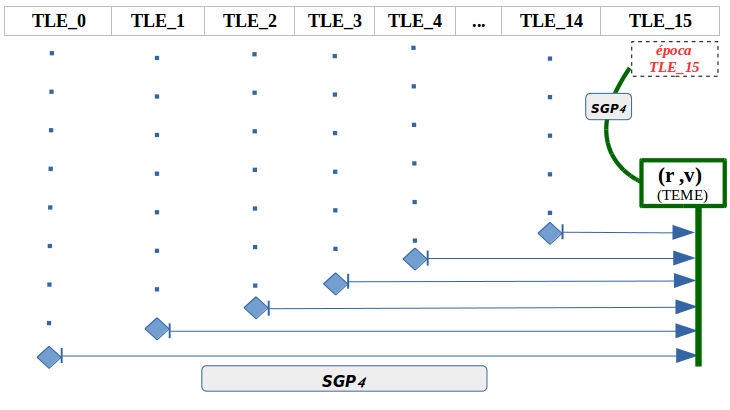
\includegraphics[width=0.8\textwidth]{imagenes/tleosw}}
\caption[M\'etodo de Osweiler, \citep{osweiler} para la generaci\'on de la matriz de covarianza]{Esquema del m\'etodo de Osweiler \citep{osweiler} para la generaci\'on de la matriz de covarianza a partir de un conjunto de TLE}
\label{fig:tleosw}
\end{figure}

Este mismo m\'etodo se aplica a la misi\'on operativa, en aquellos escenarios en los que no se tiene acceso al dato de las efem\'erides precisas, como ocurre con los casos de estudio de validaci\'on que involucran misiones operativas de otras agencias.\\

\subsection{Propagaci\'on de errores utilizando datos de TLE y efem\'erides precisas}\label{subsec:tablaprop}
Una vez que ya se conoce la matriz de covarianza del desecho para la posici\'on inicial, ser\'a necesario propagar esos errores al momento de m\'aximo acercamiento.
Dado que se desconocen los errores que introduce el propagador SGP4, fue necesario pensar una metodolog\'ia que permita hacer una estimaci\'on independiente.\\

Se propone un m\'etodo que utiliza las diferencias que resultan de los valores que ofrecen las efem\'erides precisas, en comparaci\'on con los valores que resultan de las propagaciones de TLE mediante SGP4. Se evalu\'o la tendencia en una ventana temporal de seis meses y se calcularon los valores medios de los errores, en funci\'on de la cantidad de d\'ias de propagaci\'on.

\subsubsection*{Metodolog\'ia del estudio de la propagaci\'on de errores}\label{subsec:errorProp}
Pasos que se realizan, (Fig. \ref{fig:metodotabla}):
\begin{itemize}
\itemsep0em
\item Se selecciona un intervalo de 6 meses.
\item Se extraen los productos orbitales de la misi\'on operativa tabulados cada un segundo.
\item Se solicitan los TLE de la misi\'on correspondientes al intervalo.
\item Se toma el TLE del primer d\'ia y se lo propaga cada un segundo, para los pr\'oximos 7 d\'ias.
\item Se comparan las efem\'erides precisas con los valores que resultan de los TLE propagados.
\item Se calculan las varianzas en las coordenadas R, T y N, para cada d\'ia.
\item Se toma el TLE del d\'ia siguiente y se repite el procedimiento.
\item Se realiza la estad\'istica  de las diferencias agrupadas seg\'un sean, menores a un d\'ia y hasta 6 d\'ias.
\item Se plasman los resultados en una tabla que luego ser\'a usada por ARxCODE.
\end{itemize}

\begin{figure}[!h]
\centering
\fbox{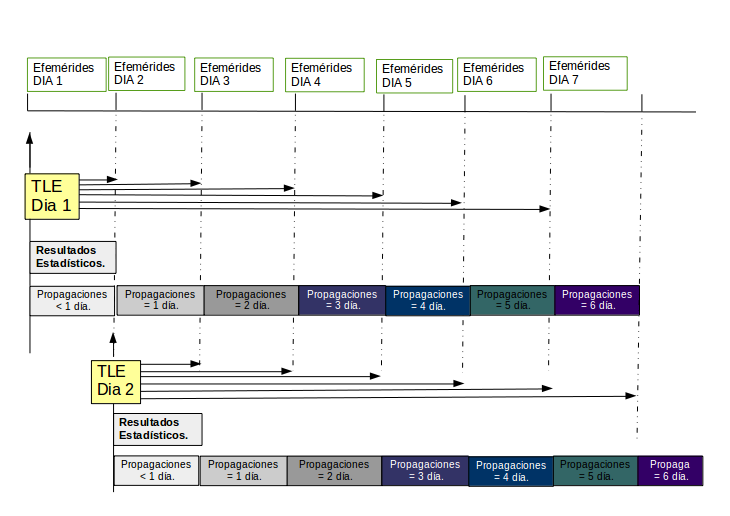
\includegraphics[width=\textwidth]{imagenes/metodoTabla}}
\caption[Descripci\'on del m\'etodo propuesto para la propagaci\'on de errores]{Esquema del m\'etodo propuesto para la estimaci\'on de la propagaci\'on de errores al utilizar TLE y el propagador SGP4. Los recuadros verdes contienen las efem\'erides precisas. Cada uno de los TLE se propagan para cada segundo, durante 7 d\'ias hacia adelante, y se comparan los valores de cada instante propagado con las efem\'erides precisas. Aqu\'i s\'olo se muestra la propagaci\'on de 2 d\'ias, pero el proceso se repite para los 6 meses del intervalo.}
\label{fig:metodotabla}
\end{figure}

A partir de las diferencias calculadas para cada segundo de cada d\'ia, se calculan valores medios y varianzas, por d\'ia.\\


\begin{figure}[!h]
\centering
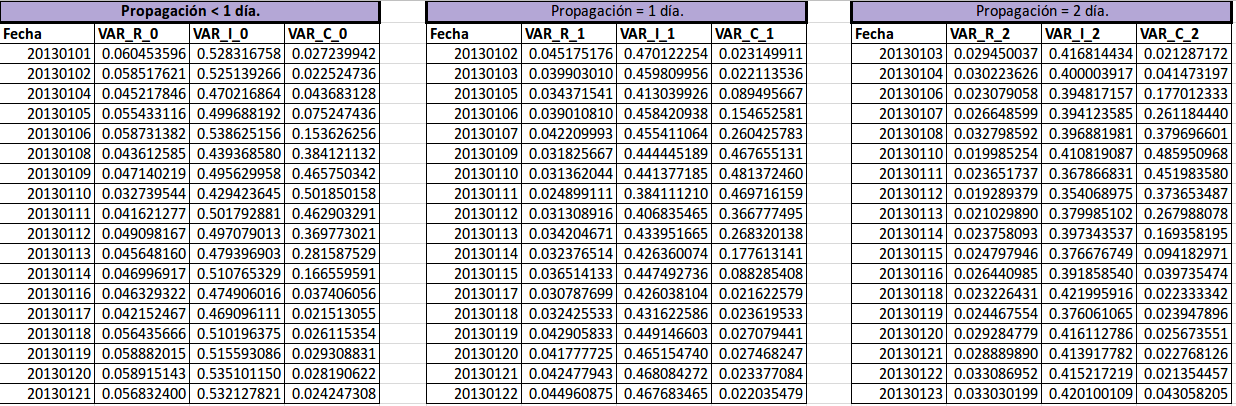
\includegraphics[width=\textwidth]{imagenes/tablacompleta}
\caption[Tabla de Estimaci\'on de errores.]{Fracci\'on de tabla con el total de datos calculados para la estimaci\'on estad\'istica. Se muestran s\'olo algunos d\'ias (primera columna de cada set) de los 6 meses, y los agrupamientos seg\'un sean respecto a propagaciones $< 1$ d\'ia, $= 1$ d\'ia o $= 2$ d\'ias}
\label{fig:tablacompleta}
\end{figure}

Luego se agrupan los valores seg\'un el intervalo de propagaci\'on, es decir, si son valores medios y varianzas de haber propagado 1, 2, 3 ... o hasta 6 d\'ias, y se toman los valores medios. Los resultados finales se plasman en una tabla cuyas columnas indican los valores medios de las varianzas por coordenada, y las filas los valores medios de las varianzas por intervalo propagado.\\

\begin{table}[!h]
\caption[Tabla con los valores medios para la propagaci\'on de errores.]{Valores medios de las varianzas para la propagaci\'on de errores. }
\begin{tabular}{l c c c}
\hline \hline
\rowcolor{yellow!35}
&$\sigma^{2}_R [km]$ &$\sigma^{2}_T [km]$ &$\sigma^{2}_N [km]$\\
\hline \hline
< 1 d\'ia & 0.05287535953&0.5110606907&0.09802202353\\

1 d\'ia & 0.03846388969&0.4517572281&0.09807457894\\

2 d\'ias & 0.02760890529&0.4086434248&0.09904162392\\

3 d\'ias & 0.01963580775&0.3765098311&0.09022336881\\

4 d\'ias & 0.01469071678&0.3577884914&0.1182060362\\

5 d\'ias & 0.01332578794&0.3557767231&0.1264764812\\

6 d\'ias & 0.01524829841&0.365815954&0.1607439516\\
\hline
\end{tabular}
\label{tab:resultatabla0}
\begin{flushleft}
\small Autor\'ia propia.
\end{flushleft}
\end{table}

De la Tabla \ref{tab:resultatabla0} se extrae que la componente T es la que mayor error introduce; con valores del orden de centenas de metros. Esto se debe a que el modelo de propagaci\'on SGP4 es d\'ebil en su representaci\'on del efecto que imprime el frenado atmosf\'erico en la componente asociada al movimiento o {\it{along-track}} T. 

\section{La probabilidad de colisi\'on}\label{sec:probcol}
Para el an\'alisis de una situaci\'on de riesgo, en general, se utilizan los par\'ametros:\\


\begin{itemize}
\itemsep0em
\item M\'inima distancia.
\item PoC.
\item M\'axima PoC.
\end{itemize}


Estos par\'ametros se calculan a partir de las \'orbitas predichas y las matrices de covarianza de los errores en el TCA (Time of Closest Approach).

Sean dos objetos; en nuestro caso una misi\'on operativa, {\it{sat}}, y un desecho, {\it{deb}}; de los cuales conocemos su posici\'on $\bar{X}_{sat0}=(\bar{x}_{sat},\bar{v}_{sat})$ y $\bar{X}_{deb0}=(\bar{x}_{deb}$,  $\bar{v}_{deb})$ y las matrices de covarianza de los errores, $C_{sat0}$, $C_{deb0}$, en un tiempo inicial,  $t_{sat0}$, y $t_{deb0}$ respectivamente. Todo referenciado al mismo sistema inercial de referencia, ya sea un sistema geoc\'entrico o \ac{ECI}; o el sistema del sat\'elite, \ac{RTN}.\\

En un planteo general, el estudio de una posible colisi\'on consiste en propagar hacia el futuro, mediante modelos (anal\'iticos y/o num\'ericos) las posiciones iniciales y las matrices de covarianza de errores; definir radios seguros (o de colisi\'on) para los objetos, y calcular la probabilidad de que la m\'inimia distancia entre ellos, sea menor a la suma de esos radios.\\

Un an\'alisis apropiado de situaciones de encuentro facilita la determinaci\'on del tiempo de m\'aximo acercamiento y las posiciones y matrices de covarianza para ese instante:  $\bar{X}_{sat}(TCA)$, $\bar{X}_{deb}(TCA)$, $C_{sat}(TCA)$, $C_{deb}(TCA)$.\\

Para su estudio, los encuentros pueden clasificarse seg\'un sean, encuentros cortos o largos. En particular en este trabajo, analizamos las situaciones de encuentros cortos considerando las hip\'otesis que propone Lei-Chen \citep{leichen}.\\

\begin{itemize}
 \item {\bf{Encuentros cortos}}: se asume que el movimiento relativo presenta comportamiento lineal durante el breve intervalo del encuentro.
 \item {\bf{Encuentros largos}}: el encuentro no es lo suficientemente corto como para considerar movimiento relativo lineal.
\end{itemize}


En los encuentros cortos puede asumirse que:\\

\begin{itemize}
\itemsep0em
 \item El movimiento relativo es lineal.
 \item Los errores en la posici\'on durante el encuentro son constantes e iguales al del error en TCA.
 \item No hay errores en la velocidad.
 \item Los errores en la posici\'on se representan con una distribuci\'on gaussiana de tres dimensiones.
\end{itemize}

La probabilidad de colisi\'on se calcula en cada caso, conociendo: las posiciones, las matrices de covarianza de ambos objetos en el instante TCA, ($\bar{X}_{sat}(TCA)$, $\bar{X}_{deb}(TCA)$, $C_{sat}(TCA)$, $C_{deb}(TCA)$) y los radios de colisi\'on respectivos, $R1$ y $R2$. En este trabajo, los radios $R1$ y $R2$  son los radios de dos esferas que envuelven a la misi\'on primaria y al desecho respectivamente. En todos los casos, el radio de la misi\'on primaria es conocido, mientras que el radio del desecho de determina a partir del seguimiento con radares, considerando la RCS (Radar Cross Section). 

\subsection*{C\'alculo de la PoC en encuentros cortos}

Distintos autores han desarrollado varios m\'etodos para el c\'alculo de la PoC (Ver tabla \ref{tab:trabajosPoc}). Todos ellos comparten las siguientes consideraciones:\\
\begin{itemize}
\itemsep0em
\item El error en la posici\'on puede representarse por una funci\'on de distribuci\'on Gaussiana en tres dimensiones (3D).
\item Tanto el objeto primario, como el desecho se mueven con movimiento rectil\'ineo de velocidad constante durante el encuentro.
\item Los errores en las velocidades se desprecian.
\item Los errores en las posiciones del objeto primario y del desecho no est\'an correlacionados.
\item Los errores en las posiciones son constantes durante el encuentro, al igual que la matrices de covarianzas correspondientes al TCA.
\end{itemize}

\begin{table}\renewcommand{\arraystretch}{1.5}
\caption[Trabajos sobre el c\'alculo de la PoC]{Distintos autores y trabajos para el c\'alculo de la Probabilidad de Colisi\'on PoC}
 \centering
  \resizebox{\linewidth}{!}{
 \begin{tabular}{cl}
 \hline \hline
 Autor/es & Metodolog\'ia\\
 \hline \hline
    Akella y Alfriend & Calcula la integral de superficie, del problema simplificado a 2D.\\
    \hline
    \multirow{4}{*}{Foster} & Calcula la integral de superficie del problema simplificado a 2D, utilizando la suma\\
    &  acumulada de anillos el\'ipticos conc\'entricos. Transforma el sistema a un sistema   \\
    & de referencia polar, e integra cada $0.5^{\circ}$ y un radio de $r_{a}/12$.\\
    & Es el m\'etodo que utiliza NASA para la ISS.\\
    \hline
    \multirow{4}{*}{Chan} & Desarroll\'o una soluci\'on anal\'itica en base a una serie infinita de\\
    &  t\'erminos que converge para la mayor\'ia de los valores m\'as comunes del problema,  \\
    &  a saber: radios combinados $r_{a}$ entre $1-100 m$, distancias m\'inimas  \\
    & de $10m-100km$ y covarianzas en el rango de $1m-10km$. \\
    \hline
    \multirow{3}{*}{Patera} & Transforma la integral de superficie a una integral de l\'inea\\
    &  de una dimensi\'on. Este nuevo planteo permite adaptar la secci\'on \\
    & de superfice a la forma de los objetos.\\
    \hline
    \multirow{2}{*}{Alfano (Serie)} & Utiliza una serie que combina las funciones error y\\
    & t\'erminos exponenciales para aproximar la integral de 2D.\\
    \hline
    \multirow{3}{*}{Alfano (Prob. M\'axima)} & Expresi\'on simplificada que permite hacer una estimaci\'on grosera\\
    & cuando no se cuenta con datos precisos de posici\'on o de la matriz de covarianza. \\
    & Utiliza una relaci\'on entre los radios combinados y la m\'inima distancia.\\
    \hline
 \end{tabular} }
 \label{tab:trabajosPoc}
\end{table}

En su mayor\'ia, los m\'etodos que se mencionan en la Tabla \ref{tab:trabajosPoc}, son aceptados en el est\'andar del mensaje de alerta para el c\'alculo de la probabilidad de colisi\'on, (Fig. \ref{fig:pagsana}).

% Los resultados del c\'alculo son sensibles a:
% 
% \begin{itemize}
% \itemsep0em
%  \item La geometr\'ia del encuentro.
%  \item La matriz de covarianza.
%  \item El tamaño de los objetos.
% \end{itemize}
  

\subsection{C\'alculo simplificado de Lei-Chen}\label{subsec:pocsimp}

En este trabajo se implement\'o la estimaci\'on de un c\'alculo simplificado para la PoC, que propone Lei-Chen junto a otros autores en el libro 
{\it{Orbital Data Applications for Space Objects. Conjunction Assessment and Situation Analysis}} \citep{leichen}.

Lei-Chen se basa en el desarrollo anal\'itco de Chan \citep{chan2003improved} y otros estudios anteriores del problema del c\'alculo de la probabilidad de colisi\'on en encuentros cortos, que reducen el problema en tres dimensiones a un plano de encuentro.
Con este planteo, se reduce el problema a calcular la integral de la funci\'on de densidad de probabilidad (PDF) en dos dimensiones, sobre el \'area de la secci\'on circular de colisi\'on que se proyecta en el plano de encuentro.\\

La secci\'on circular de colisi\'on que se proyecta en el plano de encuentro, con radio $r_{a}$, est\'a centrada en las coordenadas $\mu_{x}$, $\mu_{y}$ del plano. Las desviaciones est\'andar que resultan de la matriz combinada de covarianzas de ambos objetos, proyectadas, son $\sigma_{x}$ y $\sigma_{y}$,  (Fig. \ref{fig:planoenc}).\\

\begin{figure}[!h]
\centering
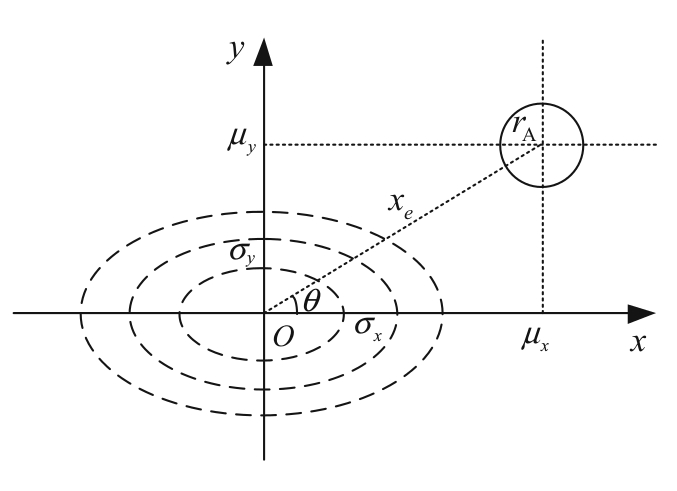
\includegraphics[width=0.6\textwidth]{imagenes/planodeencuentro}
\caption[Plano de Encuentro]{Esquematizaci\'on del plano de encuentro. Extra\'ido de Lei-Chen, \citep{leichen}.}
\label{fig:planoenc}
\end{figure}

Finalmente, la expresi\'on del c\'alculo de la integral en dos dimensiones (2D), resulta:\\

\begin{equation}
 PoC=\int \int_{(x-\mu_{x})^{2}+(y-\mu_{y})^{2}\leq r_{a}^{2}} \frac{1}{2\pi\sigma_{x}\sigma_{y}} exp [-\frac{1}{2}(\frac{\mu_{x}^{2}}{\sigma_{x}^{2}}+\frac{\mu_{y}^{2}}{\sigma_{y}^{2}}) ] dy dx
 \label{eq:pocintegral}
\end{equation}

Tomando como referencia el trabajo de Chan \citep{chan2003improved} en la b\'usqueda de una expresi\'on anal\'itica que se construye mediante una serie convergente de infinitos t\'erminos; Lei-Chen presenta una expresi\'on para el primer t\'ermino de la serie y una f\'ormula recursiva de la serie, que resulta ventajosa para los m\'etodos de programaci\'on.\\

Como resultado de su trabajo \citep{lei2009rapid}, se encuentra que si se toma el primer t\'ermino de la serie como aproximaci\'on de la integral de la PoC,  el error de truncamiento es del orden de $10^{-5}$ o menor. Si se toman los dos primeros t\'erminos, el error de truncamiento es del orden de $10^{-9}$. Es decir, que para un primer an\'alisis, resulta suficiente considerar s\'olo el primer t\'ermino de la serie, cuya expresi\'on final es:\\


\begin{equation}
 PoC= \exp[-\frac{1}{2}(\frac{\mu_{x}^{2}}{\sigma_{x}^{2}}+\frac{\mu_{y}^{2}}{\sigma_{y}^{2}})][1-\exp(\frac{r_{a}^{2}}{2\sigma_{x}\sigma_{y}})]
 \label{eq:pocexpress}
\end{equation}

Ser\'a necesario incorporar m\'as t\'erminos en aquellos casos, en los que el radio de la secci\'on circular de colisi\'on y la m\'inima distancia sean mayores a las desviaciones est\'andar.

\subsubsection*{Expresi\'on de la PoC para \'orbitas circulares}

En la mayor\'ia de los casos, las \'orbitas son circulares o casi circulares. En esta configuraci\'on  los puntos de m\'aximo acercamiento entre las \'orbitas se ubican a lo largo de la l\'inea de intercci\'on de los planos orbitales, (Fig. \ref{fig:pocorbcirc}).\\ %el m\'aximo acercamiento de los objetos ocurre siempre en posiciones cercanas a los puntos de m\'aximo acercamiento de las \'orbitas; y para las \'orbitas circulares esto se da exactamente en la l\'inea de intersecci\'on de los planos orbitales de los dos objetos, 

\begin{figure}[!h]
\begin{minipage}[t]{0.48\textwidth}
 \centering
 \fbox{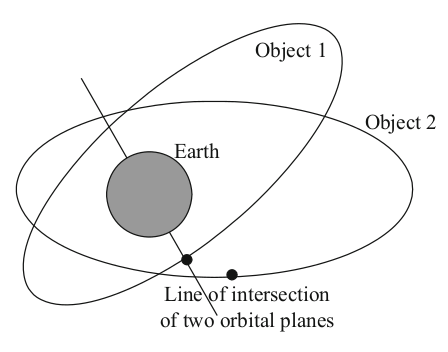
\includegraphics[width=0.8\textwidth]{imagenes/poccirc1}}
 \caption[M\'aximo acercamiento en \'orbitas circulares]{El punto de m\'aximo acercamiento en \'orbitas casi circulares ocurre siempre en puntos cercanos a la l\'inea de intersecci\'on de los planos orbitales. Extra\'ido de Lei-Chen. \citep{leichen}.}
 \label{fig:pocorbcirc}
\end{minipage}
\begin{minipage}[t]{0.48\textwidth}
 \centering
 \fbox{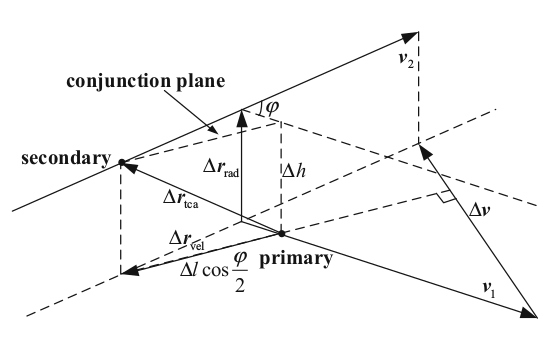
\includegraphics[width=\textwidth]{imagenes/poccirc2}}
 \caption[]{El m\'aximo acercamiento entre las \'orbitas $\Delta r_{rad}$ y el vector de m\'aximo acercamiento entre los objetos en el TCA, $\Delta r_{tca}$.}
 \label{fig:pocdistancia}
\end{minipage}
\end{figure}
 
Para el TCA, las coordenadas del centro del elipsoide de posici\'on del objeto secundario, son:\\
% 
\begin{gather}
 \mu_{x}=\Delta r_{rad}\\
 \mu_{y}=\Delta r_{vel}\\
\end{gather}
% 
Donde $\Delta r_{rad}$ es el vector de m\'aximo acercamiento entre las \'orbitas en la direcci\'on de la l\'inea perpendicular a ambas velocidades, que para el caso de \'orbitas circulares coincide con la direcci\'on radial; y $\Delta r_{vel}$ es el vector de m\'aximo acercamiento en el plano perpendicular a la direcci\'on de $\Delta r_{rad}$ (Figura \ref{fig:pocdistancia}). 

Estas expresiones, proyectadas en el sistema RSW, (Fig. \ref{fig:pocplano} y \ref{fig:pochorizontal}), resultan en:

\begin{gather}
 \mu_{x}=R\\
 \mu_{y}=\sqrt(S^{2}+W^{2})
\end{gather}

\begin{figure}[!h]
\begin{minipage}[t]{0.48\textwidth}
 \centering
 \fbox{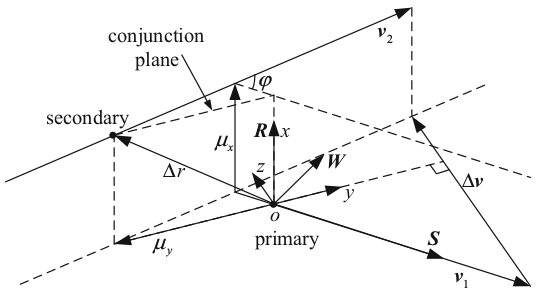
\includegraphics[width=0.8\textwidth]{imagenes/poccirc3}}
 \caption[Plano de encuentro y proyecci\'on del sistema RSW]{Definici\'on del plano de encuentro, {\it{conjuction plane}} y el sistema de coordenadas del objeto primario RSW. Extra\'ido de Lei-Chen, \citep{leichen}.}
 \label{fig:pocplano}
\end{minipage}
\begin{minipage}[t]{0.48\textwidth}
 \centering
 \fbox{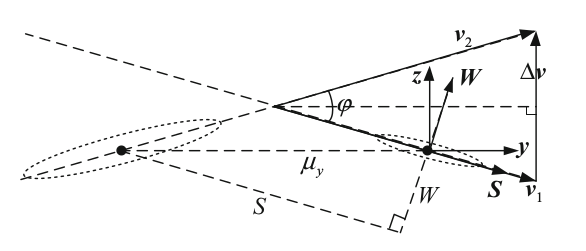
\includegraphics[width=\textwidth]{imagenes/poccirc4}}
 \caption[Proyecci\'on de los elipsoides de error al plano de encuentro]{Proyecci\'on de de los elipsoides de error al plano de encuentro. Extra\'ido de Lei-Chen, \citep{leichen}.}
\label{fig:pochorizontal}
\end{minipage}
\end{figure}

\begin{gather*}
\sigma_{x}^{2}=\sigma_{R}^{2}=\sigma_{1R}^{2}+\sigma_{2R}^{2}\\
\sigma_{y}^{2}=\sigma_{SR}^{2}=\sigma_{S}^{2}cos^{2}(\frac{\phi}{2})+\sigma_{W}^{2}sin^{2}(\frac{\phi}{2})\\
\sigma_{S}^{2}=\sigma_{1S}^{2}+\sigma_{2S}^{2}\\
\sigma_{W}^{2}=\sigma_{1W}^{2}+\sigma_{2W}^{2}\\
\end{gather*}

Donde:
\begin{itemize}
 \item $\sigma_{1R}^{2}$ y $\sigma_{2R}^{2}$  son las varianzas en la radial de ambos objetos.
 \item $\sigma_{R}^{2}$ es la suma de las varianzas $\sigma_{1R}^{2}$,$\sigma_{2R}^{2}$.
 \item $\sigma_{S}^{2}$ y $\sigma_{W}^{2}$ son las sumas de las varianzas de las componentes S y W, respectivamente.
 \item $\sigma_{SR}^{2}$ es el vector resultante de S y W, que se proyecta en la coordenada $y$ del plano de encuentro.
 \item $\phi$ es el \'angulo entre las direcciones de las velocidades de ambos objetos.
\end{itemize}


% \subsection*{M\'etodo de Akella}
% En este trabajo para el c\'alculo de la PoC se utilizar\'a el m\'etodo de Alfriend \& Akella \citep{akellaAlfriend} ya que es conceptualmente simple y aunque tiene un alto costo computacional, es realizable por las m\'aquinas actuales en tiempos menores a un segundo.\\
% 
% El mismo requiere como entradas:
% \begin{itemize}
% \itemsep0em
% \item Conocer el instante de m\'aximo acercamiento: TCA (Time of Closest Approach).
% \item La posici\'on relativa del desecho respecto al objeto primario en el TCA.
% \item La velocidad relativa del desecho respecto al objeto primario en el TCA.
% \item Las matrices de error de ambos objetos.
% \end{itemize}
% 
% En los momentos pr\'oximos al encuentro, la posici\'on relativa de riesgo $\Delta r$ puede expresarse en funci\'on de un intervalo de tiempo respecto del TCA, es decir, $\Delta t_{tca}=t-t_{tca}$.
% 
% \begin{equation}
% \Delta r(t)=\Delta r_{tca}+\Delta v_{tca}(t-t_{tca})
% \end{equation}
% 
% Las matrices de covarianza de los errores que son calculadas para un momento dado t previo al TCA, deben ser propagadas. ({\bf{ver metodolog\'ia}})
% Dado que consideramos que los errores en las posiciones de ambos objetos no est\'an correlacionadas, ambas contribuciones pueden combinarse en una \'unica matriz, a partir de la suma de ambas.
% 
% \begin{equation}
% C=C_{p}+C_{d}
% \end{equation}
% 
% De $C$ s\'olo consideraremos la submatriz superior de la izquierda de dimensiones (3x3), que corresponde a los errores en las posiciones, con un $1 \sigma$.\\
% Dado que adem\'as asumimos que los errores en la posici\'on son de distribuci\'on normal en 3D, la funci\'on densidad de probabilidad $p(\Delta r)$ en momentos pr\'oximos al m\'aximo acercamiento queda definida por la expresi\'on {\bf{eq ..bla}}:
% 
% \begin{equation}
% p(\Delta r)=\frac{1}{\sqrt((2 \pi)^3det(C))} exp[-\frac{1}{2}\Delta r^TC^{-1}\Delta r]
% \end{equation}
% 
% Sean $R_{t}$ y $R_{r}$ los radios de las esferas que encierran a nuestra misi\'on principal y al desecho de riesgo, respectivamente. Se considera una situaci\'on de {\it{encuentro}} o {\it{riesgo de colisi\'on}}, al hecho de que estas esferas se intersecten, o lo que es lo mismo, si ocurre un acercamiento dentro de una esfera de {\it{radio de colisi\'on}} $R_{c}$, secci\'on $A_{c}$,  volumen $V_{c}$.
% 
% \begin{equation}
% R_{c}=R_{t}+R_{r} \qquad A_{c}=\pi R_{C}^{2} \qquad V_{c}=\frac{4}{3} \pi R_{c}^{3}
% \end{equation}
% 
% La probabilidad de colisi\'on $P_{c}$ se calcula a partir de la integral de volumen de la funci\'on densidad de probabilidad (eq) sobre la regi\'on esf\'erica $V_{c}$, centrada en el desecho de riesgo.
% \begin{equation}
% PoC=\frac{1}{\sqrt((2\pi)^3det(C))} \int \limits_{Vc} exp[-\frac{1}{2}\Delta r^TC^{-1}\Delta r]dV
% \label{eq:poc3d}
% \end{equation}
% 
% Puede demostrarse que esta integral de volumen puede reducirse a una integral de superficie mapeando el elipsoide  de los errores en la posici\'on, en contornos el\'ipticos de probabilidad constante sobre el B-plane {\bf{(citar a Foster)}}.
% 
% El B-plane es perpendicular al vector velocidad relativa $\Delta v_{tca}$ en el momento de m\'aximo acercamiento.
% A su vez, el vector $\Delta r_{tca}$ yace en el B-plane, como deja ver la ecuaci\'on de {\bf{zero-transit of the range-rate between the two objects}}:
% \begin{equation}
% \frac{\Delta v_{tca} \Delta r_{tca}}{\Delta r_{tca}}= \dot{\rho}_{tca}=0.0 \quad \rightarrow \quad t_{tca}
% \end{equation}
% 
% Definamos los vectores directores unitarios del plano como $X_{B}$ e $Y_{B}$, de acuerdo a las expresiones:
% 
% \begin{equation}
% X_{B}=\frac{\Delta r_{tca}}{|\Delta r_{tca}|} \quad Y_{B}=\frac{(\Delta r_{tca}) \times (\Delta v_{tca})}{|(\Delta r_{tca}) \times (\Delta v_{tca})|}
% \end{equation}
% 
% 
% A partir de estos vectores unitarios, se construye la matriz de transformaci\'on $R_{X_{B},Y_{B}}$ que mapea las matrices de covarianza en tres dimensiones $C=C_{x,y,z}$ a matrices de dos dimensiones en el B-plane $C_{B}$.
% 
% \begin{equation}
% C_{B} = C_{{X_{B},Y_{B}}} = R_{X_{B},Y_{B}} C R^{T}_{X_{B},Y_{B}}\\
% \end{equation}
% 
% \begin{equation}
% R_{X_{B},Y_{B}} =
% \begin{pmatrix}
% X_{B,X} & X_{B,Y} & X_{B,Z}\\
% Y_{B,X} & Y_{B,Y} & Y_{B,Z}
% \end{pmatrix}
% \end{equation}
% 
% Los ejes principales de los contornos el\'ipticos de probabilidad constante, quedan determinados a partir de los autovalores $\lambda_{i,B}(i=1,2)$ y los autovectores $\bar{e}_{i,B}$ que resuelven la ecuaci\'on:
% 
% \begin{equation}
% (C_{B} - \lambda_{i,B} I) \bar{e}_{i,B} = \bar{0}
% \end{equation}
% 
% Donde $I$ es la matriz identidad $2x2$.
% 
% Ahora, sea la elipse que representa los errores de posici\'on de $1\sigma$ en el B-plane:\\
% 
% \begin{itemize}
% \item El {\bf{semieje mayor}} queda definido por: $a_{1\sigma,B}=\sqrt(max(\lambda_{1,B},\lambda_{2,B}))$
% \item El {\bf{semieje menor}} queda definido por: $b_{1\sigma,B}=\sqrt(min(\lambda_{1,B},\lambda_{2,B}))$
% \item La {\bf{direcci\'on del semieje mayor}} ser\'a $\bar{e}_{a,B}$, con vector unitario: $ \bar{x}_{B}=\frac{\bar{e}_{a,B}}{|\bar{e}_{a,B}|}$
% \item La {\bf{orientaci\'on de $\bar{e}_{a,B}$}} respecto a la direcci\'on de la conjunci\'on $X_{B}$ la indica el \'angulo $\Phi_{B}$ (ver \ref{fig:bplane})
% \end{itemize}
% 
% \begin{equation}
% \Phi_{B}= arccos(\bar{x}_{B},X_{B})
% \end{equation}
% 
% \begin{figure}[!h]
% \centering
% 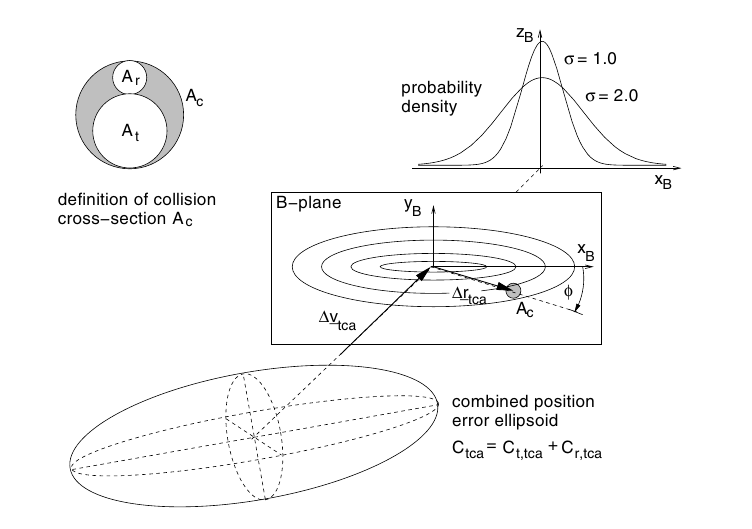
\includegraphics[width=0.5\textwidth]{imagenes/akellabplane}
% \caption{ B-plane (Adaptado de ....)}
% \label{fig:bplane}
% \end{figure}
% 
% Bien, consideremos ahora una posici\'on relativa de acercamiento $\Delta r_{B}$ ya proyectada en el B-plane. La integral de volumen de la probabilidad de colisi\'on de la Eq. \ref{eq:poc3d} se reduce a una integral de superficie sobre la secci\'on circular de colisi\'on $R_{c}$, proyectada en el B-plane y centrada a la distancia relativa predicha en el instante de m\'aximo acercamiento, $\Delta r_{tca}$
% 
% \begin{equation}
% P_{c} = \frac{1}{2 \pi \sqrt(det(C_{B}))} \int_{-R_{c}}^{+R_{c}} \int_{-\sqrt(R^{2}_{c}-x^{2}_{B})}^{+\sqrt(R^{2}_{c}-x^{2}_{B})} exp [- A_{B}] dy_{B} dx_{B}
% \end{equation}
% 
% \begin{equation}
% A_{B}=\frac{1}{2}\Delta r^{T}_{B} C^{-1}_{B} \Delta r_{B}
% \end{equation}



\section{Comunicaciones de riesgo de colisi\'on}{\label{sec:anuncio}}


A partir de los primeros accidentes y da\~nos por impactos, las agencias u organismos capaces de rastrear el ambiente espacial comenzaron a implementar sistemas de comunicaci\'on para advertir sobre posibles colisiones. Las comunicaciones, que en sus or\'igenes eran correos electr\'onicos particulares, fueron migrando a un mensaje formal y estandarizado y finalmente en Junio del 2013, el \ac{CCSDS}, public\'o el mensaje est\'andar recomendado que se utiliza en la actualidad, el: \ac{CDM} \citep{CDM}.\\

El {\it{CCSDS 508.0-B-1, Conjunction Data Message Recommended Standard}} describe en detalle la estructura del formato recomendado, aunque no propone formas de intercambio, dejando a las partes la potestad de acordar las distintas maneras de realizar la comunicaci\'on de los mismos, que, deber\'an ser detalladas en el documento de interfaces (ICD).\\

\subsection{El mensaje de alerta CDM}\label{subsec:cdm}

Es un mensaje estandarizado para el intercambio de informaci\'on entre los organismos capaces de detectar acercamientos y los due\~nos y/o operadores de los objetos involucrados en el encuentro.\\

Los CDM se env\'ian 72 horas antes del encuentro a los operadores a cargo y/o se disponibilizan en la p\'agina de Space-track para usuarios con permisos especiales. Los mismos se generan y se distribuyen de acuerdo a ciertos criterios.\\


\underline{Criterios de generaci\'on y env\'io del CDM}
\begin{itemize}
\item Para las {\bf{\'orbitas bajas}}, se consideran las situaciones en las que la m\'inima distancia total es menor a 1 kil\'ometro y la distancia relativa en la componente radial es menor a los 200 metros.\\

\item Para las regiones de los {\bf{sat\'elites geoestacionarios o las regiones medias}}, se env\'ian mensajes si la m\'inima distancia total es menor a los 10 kil\'ometros.\\
\end{itemize}


Su formato estandarizado unifica la informaci\'on que all\'i se publica y facilita la interoperatibilidad sin ambig\"{u}edades. Su estructura est\'a pensada para que sea de f\'acil interpretaci\'on tanto para personas como para m\'aquinas. Esto permite a los centros de control de las operaciones, la automatizaci\'on de los procesos de recepci\'on de los mensajes y ofrece la informaci\'on preprocesada, dejando m\'as tiempo para la toma de decisiones.\\

Son exclusivamente informativos, no imprimen recomendaciones ni sugerencias de acci\'on.
Y es importante destacar, que los centros de c\'omputo que los generan, no siempre cuentan con la informaci\'on de las pr\'oximas maniobras planificadas para los sat\'elites.\\

Es un mensaje codificado en formato ASCII, que puede distribuirse mediante un texto plano \ac{KVN}, o por medio de un \ac{XML}. Contiene la m\'inima distancia, la PoC, el TCA y las posiciones y velocidades relativas en el momento de m\'inima distancia; entre muchos otros \citep{CDM}.\\

Ofrece la siguiente informaci\'on de un \'unico encuentro entre dos objetos: {\it{Object1}} y {\it{Object2}}:
\begin{itemize}
\item Las posiciones de  {\it{Object1}} y  {\it{Object2}} en el instante de m\'aximo acercamiento TCA en alguno de los sistemas de referencia m\'as utilizados (Sec. \ref{subsec:sistRef}).
\item Las covarianzas de las posiciones de los objetos en el instante TCA, tomando como referencia el centro de uno de ellos.
\item La posici\'on y velocidad relativa del {\it{Object2}} respecto al centro del {\it{Object1}}.
\item Informaci\'on relevante respecto a c\'omo fueron obtenidos los datos anteriores.
\end{itemize}


\subsubsection*{Estructura general del formato KVN}
El CDM en su formato KVN, consiste en un texto plano, con palabras claves o {\it{keywords}}, con su valor correspondiente.\\
El mensaje contiene una {\it{keyword}} por l\'inea, y el orden en que se presentan es fijo y est\'a determinado por el est\'andar, respetando la siguiente estructura:

\begin{itemize}
\itemsep0em
\item Un Encabezado.
\item Metadatos y datos relativos (datos que describen relaciones entre los objetos).
\item Metadatos (datos respecto a c\'omo fueron creados los objetos).
\item Datos de cada uno de los objetos.
\item Comentarios opcionales.
\end{itemize}

Ejemplo con un peque\~no segmento:\\


\fbox{\parbox[b]{\linewidth}{
\begin{tabular}{llc}
CREATION\_DATE  &= 2010-03-12T22:31:12.000&\\
ORIGINATOR &= JSPOC& \\
MESSAGE\_FOR &= SATELLITE A&\\
MESSAGE\_ID &= 201113719185&\\
TCA &= 2010-03-13T22:37:52.618&\\
MISS\_DISTANCE &= 715 &[m] \\
RELATIVE\_SPEED &= 14762& [m/s] \\
RELATIVE\_POSITION\_R &= 27.4 & [m] \\
RELATIVE\_POSITION\_T &= -70.2 &[m] \\
RELATIVE\_POSITION\_N &= 711.8& [m]\\
...& ... & \\
COLLISION\_PROBABILITY &= 4.835E-05& \\
COLLISION\_PROBABILITY\_METHOD &= FOSTER-1992&\\ 
\end{tabular}
}}

\subsubsection*{Estructura general del formato XML}
El CDM en su formato \ac{XML} proporciona un m\'etodo est\'andar para acceder a la informaci\'on, facilitando el intercambio de datos electr\'onicos. Su estructura define el tipo de informaci\'on que hay en el documento, acelerando los procesos de b\'usqueda.\\
El XML del CDM, se agrupa como se muestra a continuaci\'on:

\begin{verbbox}
<header>
</header>
<body>
  <relativeMetadataData>
  </relativeMetadataData>
  <segment>
    <metadata>
    </metadata>
    <data>
    </data>
  </segment>
  <segment>
    <metadata>
    </metadata>
    <data>
    </data>
  </segment>
</body>\\
\end{verbbox}

\begin{center}
\fbox{\parbox[b]{0.5\linewidth}{
\theverbbox }}
\end{center}


\subsubsection*{Ejemplo de CDM}
A continuaci\'on se muestra un fragmento de ejemplo de un CDM en formato XML. Un ejemplo completo se adjunta en el Ap\'endice \ref{App2}.\\

\lstset{language=XML,basicstyle=\small}
\begin{lstlisting}
<?xml version="1.0" encoding="UTF-8"?>
<cdm xmlns:xsi="http://www.w3.org/2001/XMLSchema-instance"
xsi:noNamespaceSchemaLocation=
"http://sanaregistry.org/r/ndmxml/ndmxml-1.0-master.xsd"
id="CCSDS_CDM_VERS" version="1.0">
<header>
<COMMENT>Sample CDM - XML version</COMMENT>
<CREATION_DATE>2010-03-12T22:31:12.000</CREATION_DATE>
<ORIGINATOR>JSPOC</ORIGINATOR>
<MESSAGE_FOR>SATELLITE A</MESSAGE_FOR>
<MESSAGE_ID>20111371985</MESSAGE_ID>
</header>
<body>
<relativeMetadataData>
<COMMENT>Relative Metadata/Data</COMMENT>
<TCA>2010-03-13T22:37:52.618</TCA>
<MISS_DISTANCE units="m">715</MISS_DISTANCE>
<RELATIVE_SPEED units="m/s">14762</RELATIVE_SPEED>
<relativeStateVector>
<RELATIVE_POSITION_R units="m">27.4</RELATIVE_POSITION_R>
<RELATIVE_POSITION_T units="m">-70.2</RELATIVE_POSITION_T>
<RELATIVE_POSITION_N units="m">711.8</RELATIVE_POSITION_N>
<RELATIVE_VELOCITY_R units="m/s">-7.2</RELATIVE_VELOCITY_R>
<RELATIVE_VELOCITY_T units="m/s">-14692.0</RELATIVE_VELOCITY_T>
<RELATIVE_VELOCITY_N units="m/s">-1437.2</RELATIVE_VELOCITY_N>
</relativeStateVector>
<START_SCREEN_PERIOD>2010-03-12T18:29:32.212</START_SCREEN_PERIOD>
<STOP_SCREEN_PERIOD>2010-03-15T18:29:32.212</STOP_SCREEN_PERIOD>
<SCREEN_VOLUME_FRAME>RTN</SCREEN_VOLUME_FRAME>
<SCREEN_VOLUME_SHAPE>ELLIPSOID</SCREEN_VOLUME_SHAPE>
<SCREEN_VOLUME_X units="m">200</SCREEN_VOLUME_X>
<SCREEN_VOLUME_Y units="m">1000</SCREEN_VOLUME_Y>
<SCREEN_VOLUME_Z units="m">1000</SCREEN_VOLUME_Z>
<SCREEN_ENTRY_TIME>2010-03-13T20:25:43.222</SCREEN_ENTRY_TIME>
<SCREEN_EXIT_TIME>2010-03-13T23:44:29.324</SCREEN_EXIT_TIME>
<COLLISION_PROBABILITY>4.835E-05</COLLISION_PROBABILITY>
<COLLISION_PROBABILITY_METHOD>FOSTER-1992
</COLLISION_PROBABILITY_METHOD>
</relativeMetadataData>
\end{lstlisting}

A diferencia de los mensajes estandarizados anteriores, como el CSM:{\it{Conjunction Summery Message}}, el CDM ofrece un valor estimado para la PoC e indica el m\'etodo que se utiliz\'o para calcularlo. Estos m\'etodos (Fig. \ref{fig:pagsana}), son adem\'as los m\'etodos que el est\'andar sugiere para la implementaci\'on de los c\'alculos de PoC.\\

\begin{figure}[!h]
\centering
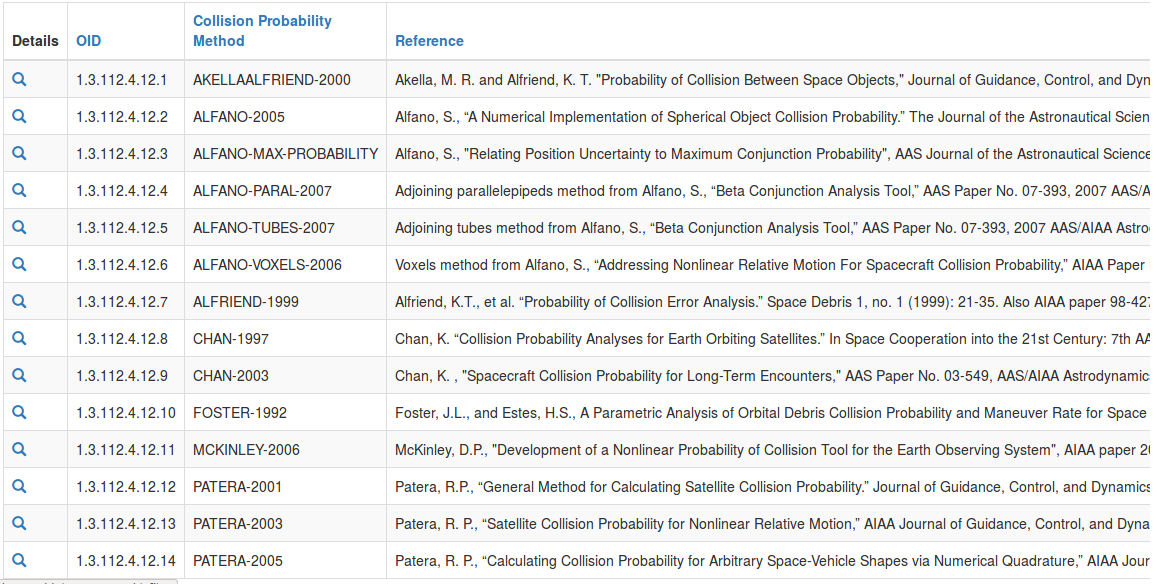
\includegraphics[width=\textwidth]{imagenes/sanaPoCmetodos}
\caption[M\'etodos de c\'alculo de PoC - (Sitio Web SANA)]{ La imagen es una impresi\'on de pantalla de la Secci\'on Probabilidad de Colisi\'on, del sitio SANA: \textcolor{blue}{http://sanaregistry.org/r/ndmxml/ndmxml-1.0-cdm-1.0.xsd}, que se indica en el est\'andar del CCSDS, para la descripci\'on de los esquemas del formato XML del CDM.}
\label{fig:pagsana}
\end{figure}

\section{Resumen}
A partir de la recepci\'on de informaci\'on respecto de una posible colisi\'on, ya sea mediante un mensaje estandarizado CDM o mediante el ingreso manual, se inicia un an\'alisis de la situaci\'on.\\
A tal fin, (Fig. \ref{fig:flujomain}):\\

\begin{itemize}
\itemsep0em
\item Se identifican los objetos involucrados, y se extra su identificador de NORAD y el TCA.
\item Se solicitan los TLE de los \'ultimos 15 d\'ias m\'as pr\'oximos a la fecha del encuentro, para el desecho y para la misi\'on operativa en caso de no contar con datos m\'as precisos. Si para la misi\'on operativa se contara con productos orbitales propios se utilizar\'an los errores calculados asociados a los mismos.
\item Se calcula la matriz de covarianza con el m\'etodo de Osweiler, \citep{osweiler} para el desecho (y para la misi\'on si los datos orbitales de la misma no se conocieran).
\item Se propagan ambas matrices hasta el TCA utilizando los datos estad\'isticos de la tabla generada, seg\'un la cantidad de d\'ias que se necesite propagar.
\item Se proyectan los distintos par\'ametros a un plano de encuentro que simplifica los c\'alculos.
\item Se calcula la probabilidad de colisi\'on mediante la expresi\'on aproximada de Lei-Chen, \citep{leichen}.
\end{itemize}

\begin{figure}[!h]
\centering
\fbox{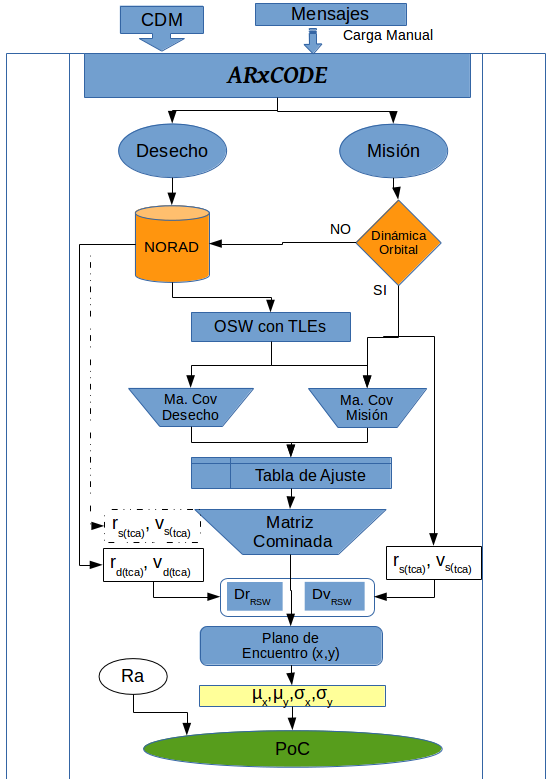
\includegraphics[width=0.7\textwidth]{imagenes/flujomain}}
\caption[Esquema del Procedimiento General del c\'alculo de PoC]{Esquema del Procedimiento General del c\'alculo de PoC}
\label{fig:flujomain}
\end{figure}

\endinput